\begin{frame}[c]
	\myframetitle{Task 2 - Crawler}{Introduction}
	\begin{itemize}
		\fatitem{Implemented in Scala}
		\fatitem{Currently, runs in a single thread.}
		\begin{itemize}
			\item Therefore we need not to worry about to many access on the same host
			\item But it can be easily moved to multithread with the Akka middleware
		\end{itemize}
		\fatitem{Started crawling at \url{http://news.google.de}}
		\fatitem{Indexed 1000 pages with BFS queue and DFS queue}
	\end{itemize}
\end{frame}

\begin{frame}[c]
	\myframetitle{Task 2 - Crawler}{New URLs found}
	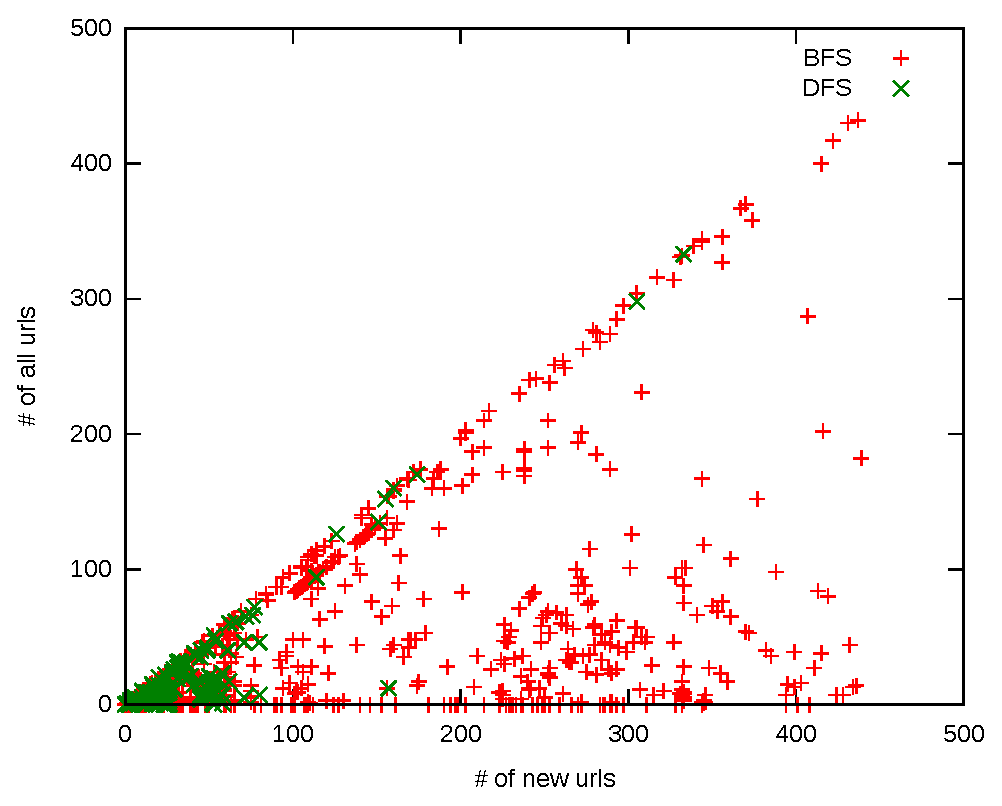
\includegraphics[width=25em]{../crawler/src/main/resources/results/bfs/newVsFoundUrls.eps} 
\end{frame}

\begin{frame}[c]
	\myframetitle{Task 2 - Crawler}{URLs per Page Statistics}
	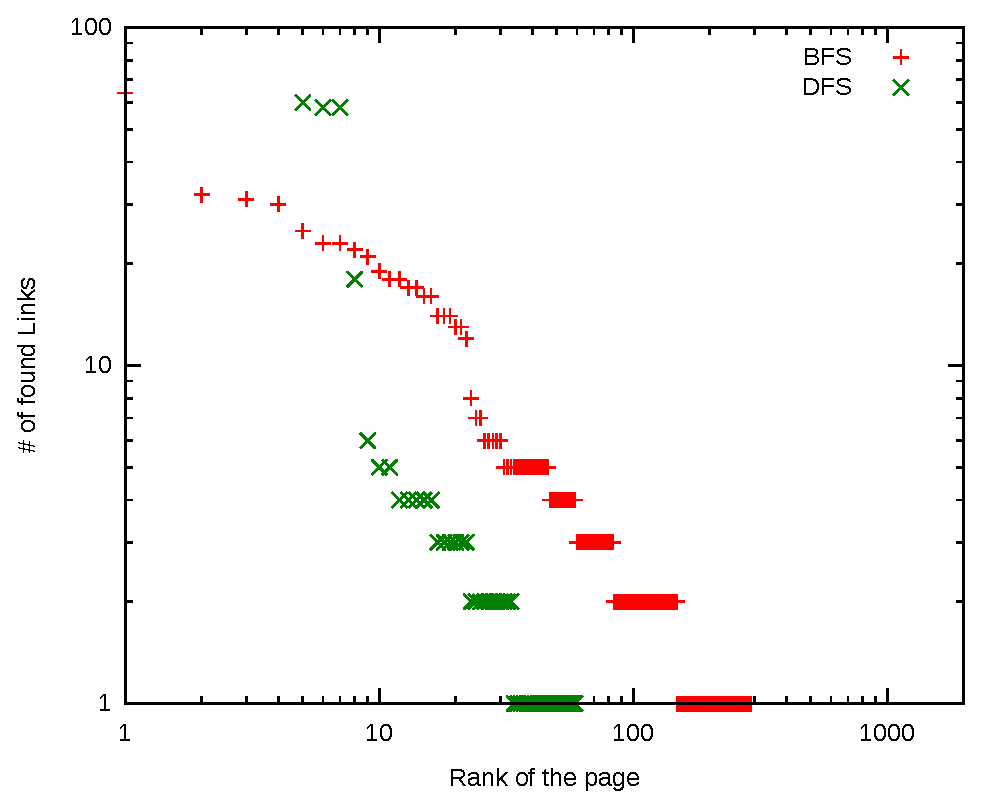
\includegraphics[width=26em]{../crawler/src/main/resources/results/bfs/histogram.eps} 
\end{frame}

\begin{frame}[c]
	\myframetitle{Task 2 - Crawler}{Frequency of links}
	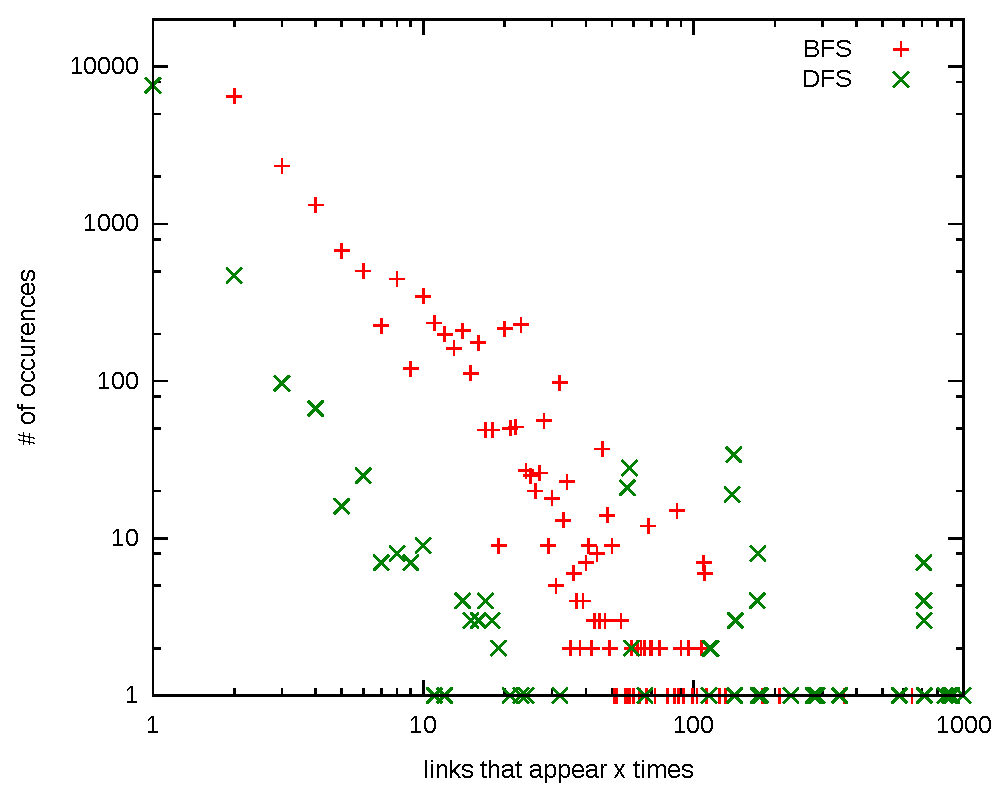
\includegraphics[width=26em]{../crawler/src/main/resources/results/bfs/distLinks.eps} 
\end{frame}

\begin{frame}[c]
	\myframetitle{Task 2 - Crawler}{Further results}

\begin{table}
\begin{tabular}{|c|c|}
\hline \textbf{BFS} & \textbf{DFS} \\ 
\hline 136 & 20 \\ 
\hline 
\end{tabular}
\caption{Different Hosts found}
\end{table}

\begin{table}
\begin{tabular}{|c|c|c|}
\hline \textbf{Language} & \textbf{DFS} & \textbf{BFS} \\ 
\hline german & 55 & \textit{935} \\ 
\hline english & \textit{943} & 43 \\ 
\hline french & 0 & 1 \\ 
\hline portuguese & 0 & 1 \\ 
\hline <unknown> & 2 & 20 \\ 
\hline $\sum$ & 1000 & 1000 \\
\hline 
\end{tabular}
\caption{Found languages in all pages}
\end{table}
\end{frame}

\begin{frame}[c]
	\myframetitle{Task 2 - Crawler}{Experiences}
	\begin{itemize}	
	\fatitem{With Javas \texttt{URL} class a URL can easily brought to the same form}
	\fatitem{But it has problems with \texttt{javascript:} and other \textit{''protocols''}}
	\fatitem{Solution: simple wrap with a try catch block}
	\fatitem{For crawling exception handling is a must! Else the crawler will stop in near time}
	\end{itemize}
\end{frame}